\chapter{矩阵乘GPU实现}\label{chap:GEMMGPU}

我们使用外积(outer product)法计算矩阵乘。因为外积法比內积法(inner product)在GPU上的并行性好。例如,我们要计算下面的矩阵乘法C=AxB。使用內积法,我们需要按照下面的公式计算:

\begin{equation}
\label{eq:innerproduct}
C[i][j]=\sum_{k}A[i][k]B[k][j]
\end{equation}

我们可以并行的计算所有的乘法,但不能并行的计算加法。即使我们可以使用reduction来快速计算加法,但仍然会产生很多空闲的线程。这样,由于任务划分的不均衡,会使得计算性能大大降低。然而,如果我们用外积法来代替內积法,将会很大程度上缓解负载不均衡带来的性能损失。下面是外积法的计算公式:

\begin{equation}
\label{eq:outerproduct}
C^{(k)}=A[:][k]B[k][:], C=\sum_{k}C^{(k)}
\end{equation}

在计算A[:][k]B[k][:]时,每个线程只需负责读取A的一个小块和B的一个小块,来计算对应C的一个小块;每个线程可以独立的将当前计算得到的C的一小块的部分和累加到对应C的一小块上。当C的部分和全部都累加起来时,我们一次性写回C到全局内存。

在算法设计上,我们采用外积法, A矩阵列优先存储,B矩阵行优先存储, 图\ref{fig:outer_product}为一个block中的线程读取A,B中的数据块, 和对应到C矩阵的输出

问题定义: C = A * B, A大小为MxK, B为KxN, C为MxN 

矩阵乘外积法: 我们用A矩阵的一列乘以B矩阵的一行,沿着K方向做累加,可以计算出结果C(图\ref{fig:outer_product})。

\section{矩阵乘外积法算法描述}

\begin{algorithm}[htbp]
	\small
	\caption{GEMM algorithm}\label{alg:gemm}
	\begin{algorithmic}[1]
		%\Procedure{Euclid}{$a,b$}\Comment{The g.c.d. of a and b}
		\State preload block of A, B
		\While{one more valid block of A, B exists}
		\State load block of A, B from global memory to registers
		\State store block of A, B from registers to shared memory
		\State load block of A, B from shared memory to registers
		\State compute block of C in registers
		\EndWhile\label{gemmendwhile}
		\State store C from registers to global memory
		%\EndProcedure
	\end{algorithmic}
\end{algorithm}


在算法执行上,我们经过下面的步骤:

(1)	数据预取, 从全局内存读取A,B矩阵数据块到寄存器

(2) 循环开始:

   (2.1)从全局内存读取A,B数据块到寄存器

   (2.2)将读取到寄存器的数据写回的共享内存

   (2.3)从共享内存读取A,B数据块到寄存器

   (2.4)在寄存器中计算结果C

直到所有的A,B数据块都读取完

(3)  最后把C的结果从寄存器写回到全局内存


\section{从全局内存读取数据到共享内存}
全局内存是对所有线程可见,共享内存是对一个线程块里的线程是可见的,寄存器是对线程私有的。从全局内存读取数据到寄存器,然后到共享内存,是为了通过数据分享共享内存的数据,减少慢速的全局内存的访问次数,改为共享内存的访问。展示了线程块从矩阵A和B读取数据到共享内存的过程。线程块分别从矩阵A和矩阵B读取bmxbk和bkxbn的数据,然后使用外积法计算。为了隐藏全局访存的延迟,我们采用软流水和共享内存双缓冲机制。共享分块的大小与GPU上的计算资源如寄存器大小和共享内存大小有关。由于指令不能直接从全局访存读取到共享内存,需要寄存器中转,因此需要分两个步骤。

\begin{figure}[htbp]
	\centering
	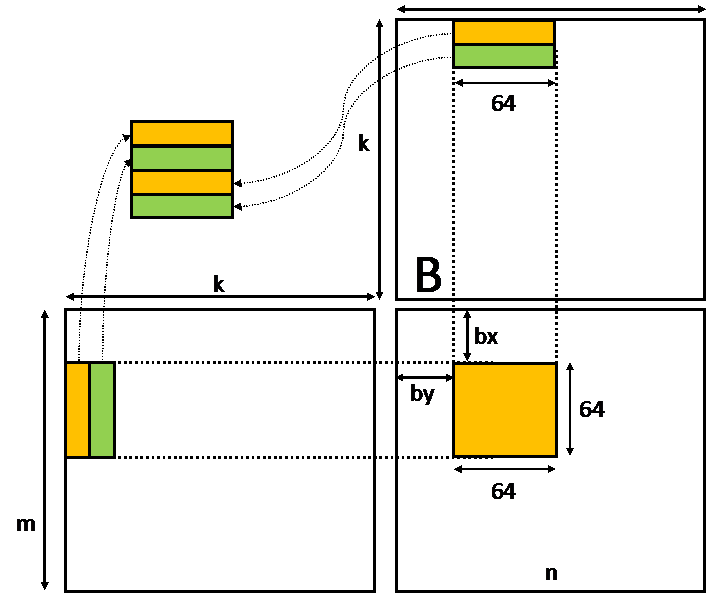
\includegraphics[width=0.50\textwidth]{outer_product}
	\bicaption{矩阵乘外积法图示}{Illustration of Outer-product matrix multiplication method}
	\label{fig:outer_product}
\end{figure}

\subsection{线程到数据的映射}

\begin{figure}[htbp]
	\centering
	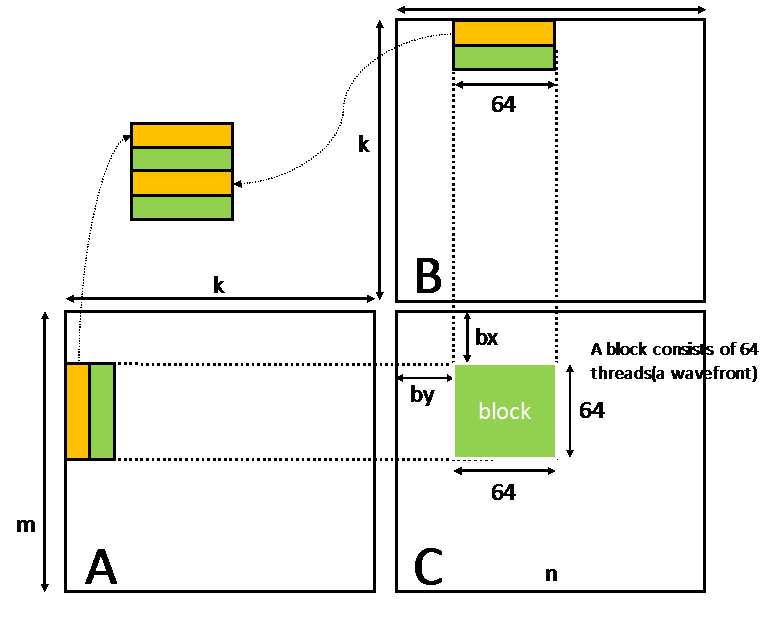
\includegraphics[width=0.50\textwidth]{thread_to_data}
	\bicaption{线程到数据映射}{Thread-to-data mapping}
	\label{fig:thread_to_data}
\end{figure}

64个线程(即一个wavefront)组成一个block,每个线程计算8x8的输出,一个block共计算64x8x8=64x64的输出(如图\ref{fig:thread_to_data})。

\begin{figure}[htbp]
	\centering
	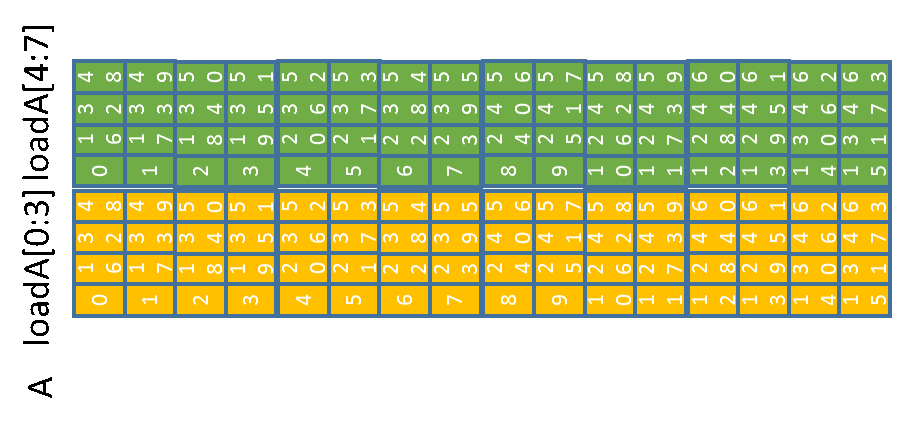
\includegraphics[width=0.50\textwidth]{global_A}
	\bicaption{从全局内存读取A矩阵数据到寄存器}{Thread-to-data mapping}
	\label{fig:global_A}
\end{figure}

\begin{figure}[htbp]
	\centering
	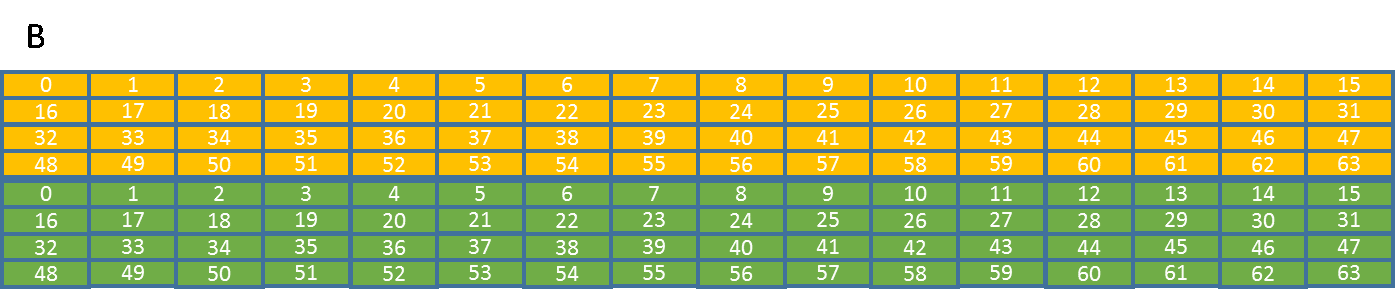
\includegraphics[width=0.50\textwidth]{global_B}
	\bicaption{从全局内存读取B矩阵数据到寄存器}{Thread-to-data mapping}
	\label{fig:global_B}
\end{figure}

A(表示保存A矩阵数据的寄存器) : 从全局内存读A数据到寄存器(如图\ref{fig:global_A})

B(表示保存B矩阵数据的寄存器) : 从全局内存读B数据到寄存器(如图\ref{fig:global_B})

图中,小方格中的数字表示threadblock中的线程号。黄色表示已经把全局内存中的数据加载到了寄存器,绿色表示下一次计算需要用到的数据(还没加载好)。黄色和绿色构成寄存器双缓冲。

\begin{figure}[htbp]
	\centering
	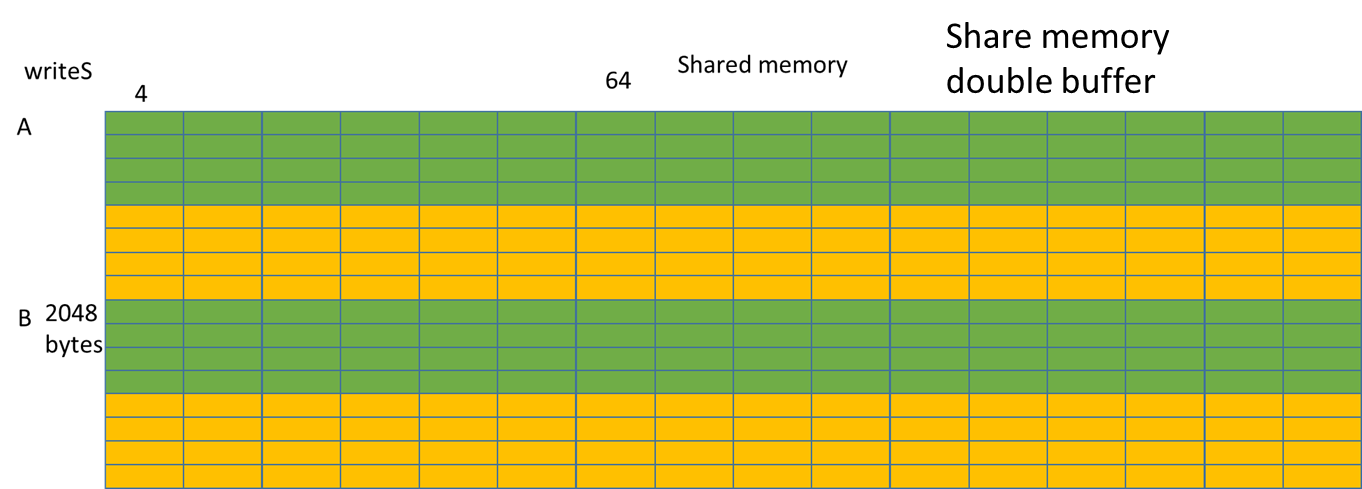
\includegraphics[width=0.50\textwidth]{writeS}
	\bicaption{写回A,B数据到共享内存}{Thread-to-data mapping}
	\label{fig:writeS}
\end{figure}

将寄存器中读好的A,B写回到局部共享内存。图\ref{fig:writeS}中绿色表示正在从寄存器写回数据到局部共享内存,黄色表示下一次要写回到局部共享内存的地址。黄色和绿色构成局部共享内存双缓冲。


\section{从共享内存读取数据到寄存器并计算}
\begin{figure}[htbp]
	\centering
	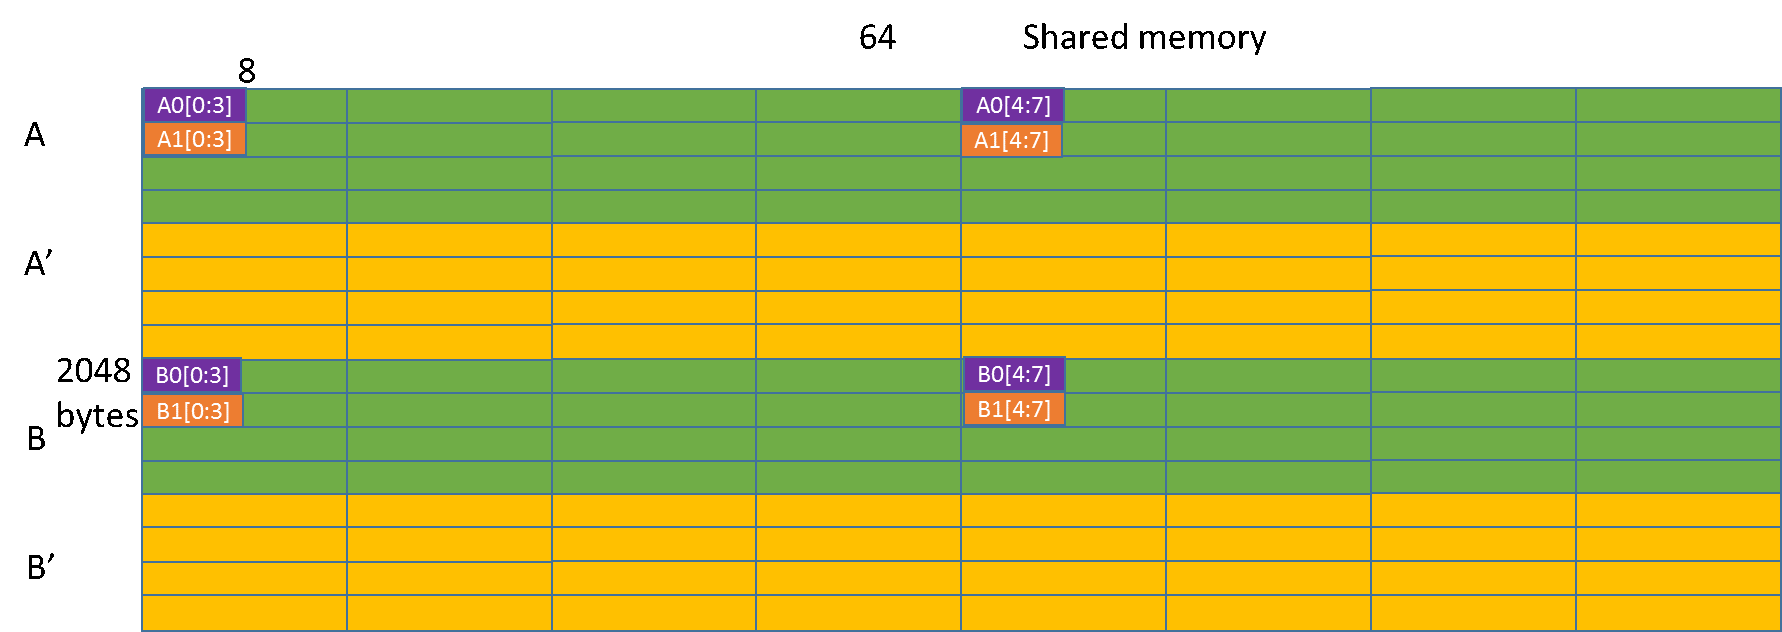
\includegraphics[width=0.50\textwidth]{readS}
	\bicaption{从共享内存读取A,B数据到寄存器}{Thread-to-data mapping}
	\label{fig:readS}
\end{figure}

接下来就可以计算矩阵C了。图\ref{fig:readS}中紫色和橙色表示0号线程从局部共享内存要读取的数据。由于我们前面讲到了循环展开8次,紫色表示偶数次要读取的数据,橙色表示奇数次读取的数据绿色表示数据已经在共享内存中了,可以直接读取,黄色表示双缓冲的另外一半。

\begin{figure}[htbp]
	\centering
	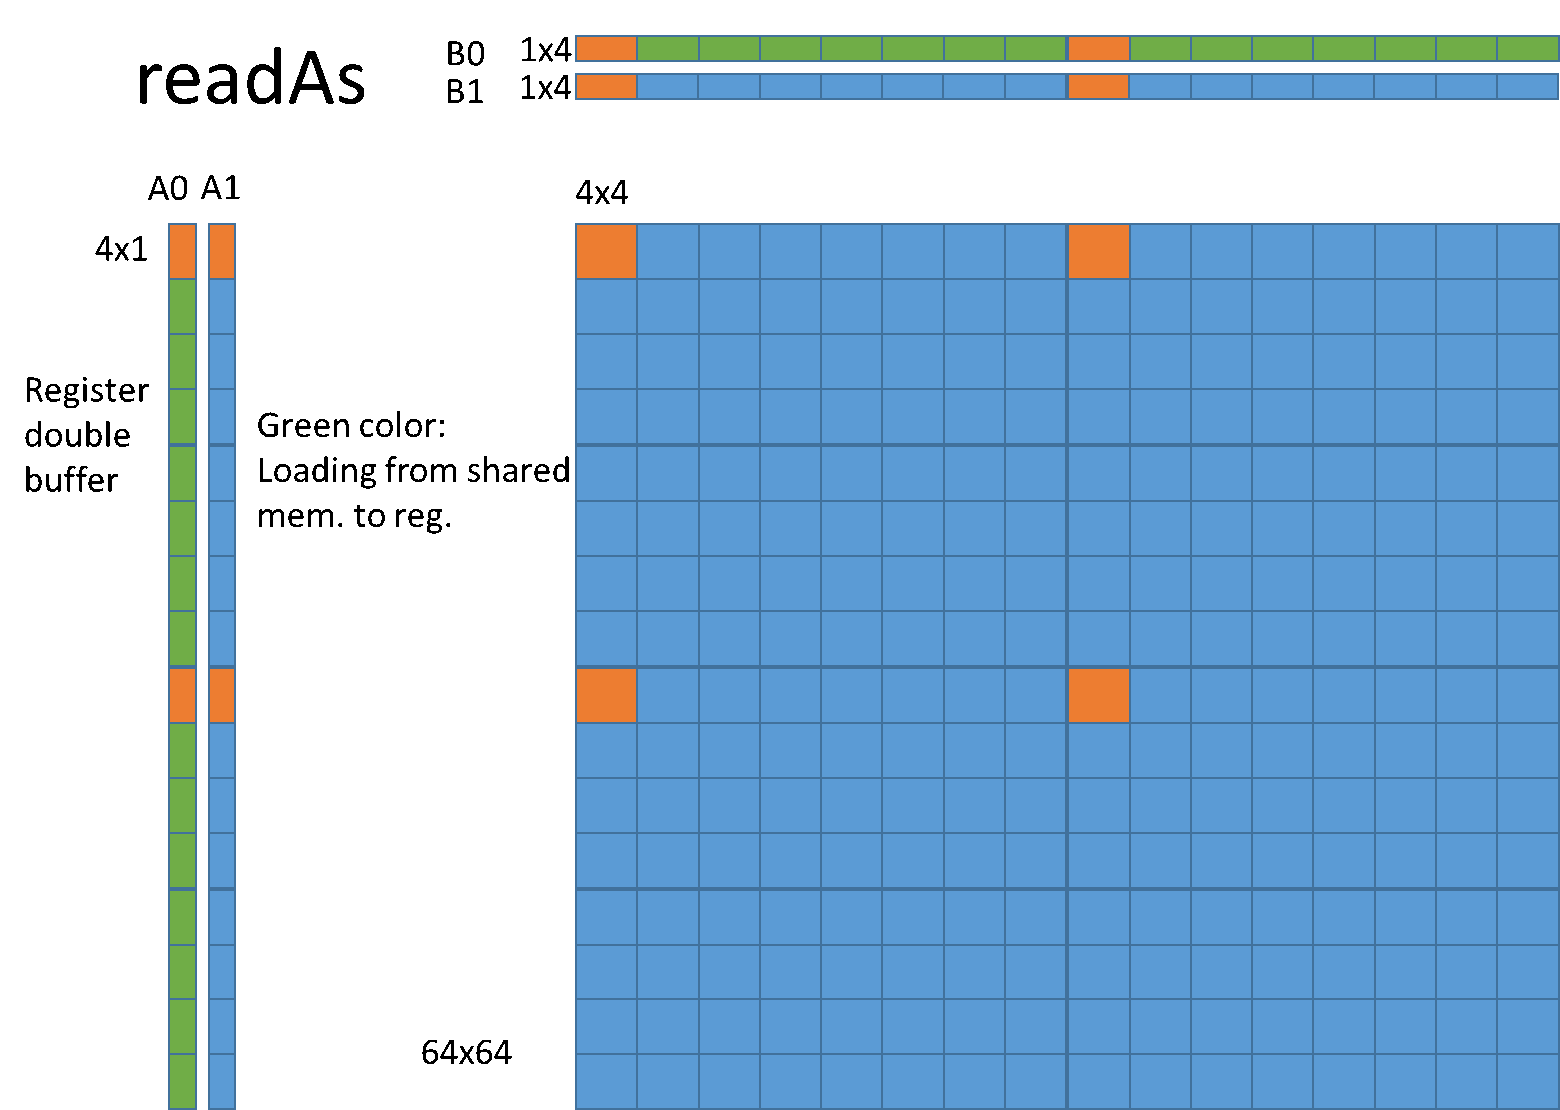
\includegraphics[width=0.50\textwidth]{threadblock}
	\bicaption{一个threadblock中的计算任务}{Thread-to-data mapping}
	\label{fig:threadblock}
\end{figure}

从block的角度观察每个线程的计算任务(如图\ref{fig:threadblock})。现在从一个block的角度来观察每个线程计算C的方式,这里一个block由一个wavefront组成,即64个线程, 一个block总共计算64x64个C中元素。图中橙色部分表示0号线程的计算任务,0号线程计算8x8的C,为了线程的负载均衡,这里将8x8分成4个4x4。
这里总结一下:我们用了到数据预取,寄存器双缓冲,局部共享内存双缓冲,bank冲突消除,负载均衡,这些优化方法


\section{将C矩阵从寄存器写回数据到全局内存}

通过乘加运算得到最终的结果C矩阵后,一般有两种方式将结果写回全局内存。第一种是先将C矩阵从寄存器写回到共性内存,然后再写回到全局内存;第二种是直接将C矩阵从寄存器写回到全局内存。
我们首先做4个v\_mul操作,将结果乘以系数alpha。然后用指令tbuffer\_store\_format\_xyzw依次写回4个结果。一个block总共需要写回64个元素,每4条v\_mul指令之间插入一条tbuffer\_store\_format\_xyzw指令。所有block并发执行,将整个C矩阵写回到全局内存。


\section{本章小结}
本章主要讲述了矩阵乘GPU实现的算法和具体实现步骤。描述了矩阵乘外积法的执行过程,并分析了外积法相比于內积法的优势。通过三个步骤讲述了外积法矩阵乘计算过程中,数据的搬运和计算的执行过程。为下一章节讲述矩阵乘调优过程做铺垫。